\begin{figure*}[t]
    \centering
    \begin{subfigure}[t]{0.5\textwidth}
        \centering
        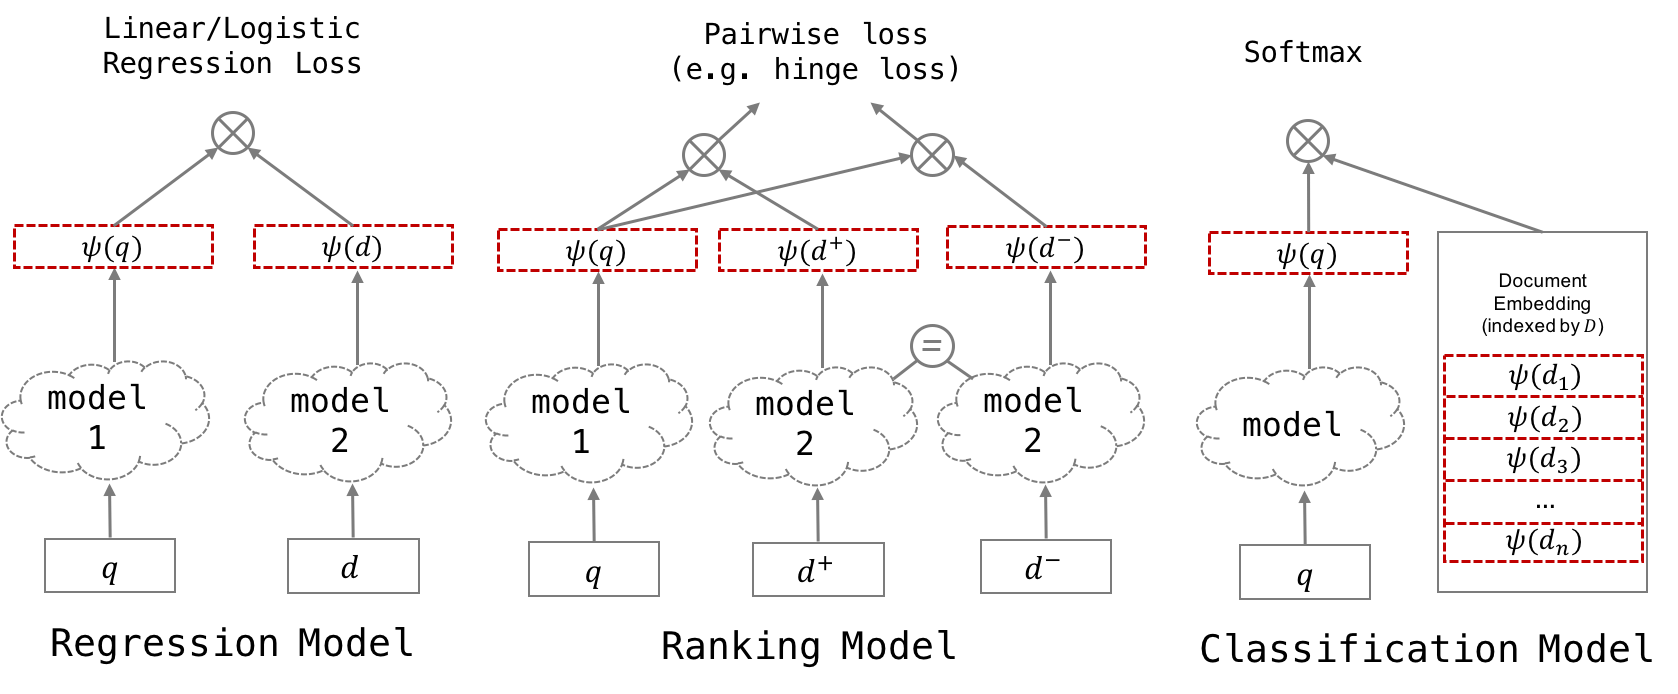
\includegraphics[height=3.5cm]{Images/O_1_Models.png}
        \caption{\label{fig:o_1_models}Constant time late combining models}
    \end{subfigure}%
    ~ 
    \begin{subfigure}[t]{0.25\textwidth}
        \centering
        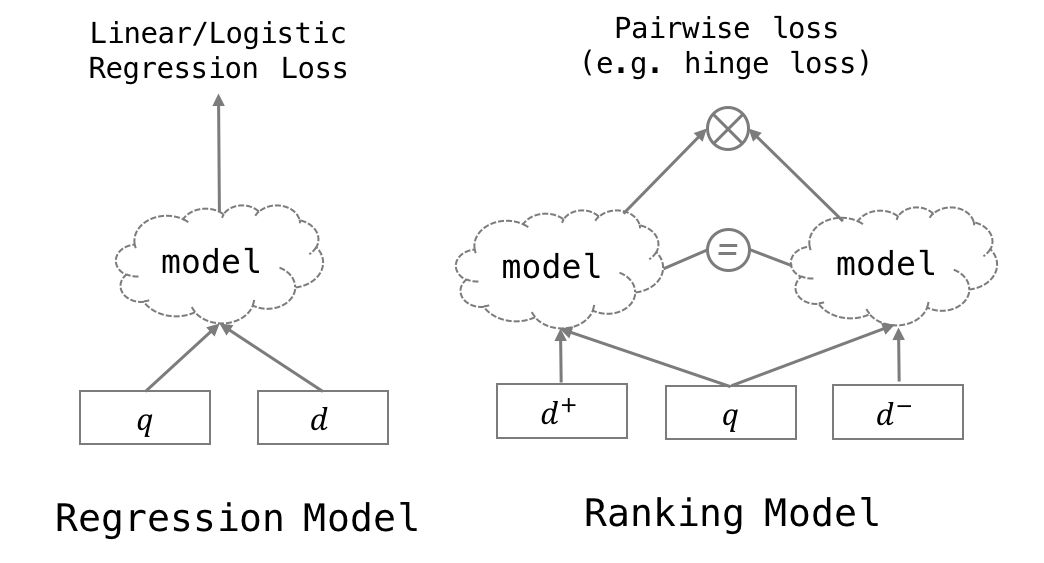
\includegraphics[height=3cm]{Images/O_n_Models.png}
        \caption{\label{fig:o_n_models}Linear time early combining models}
    \end{subfigure}%
    ~
    \begin{subfigure}[t]{0.20\textwidth}
        \centering
        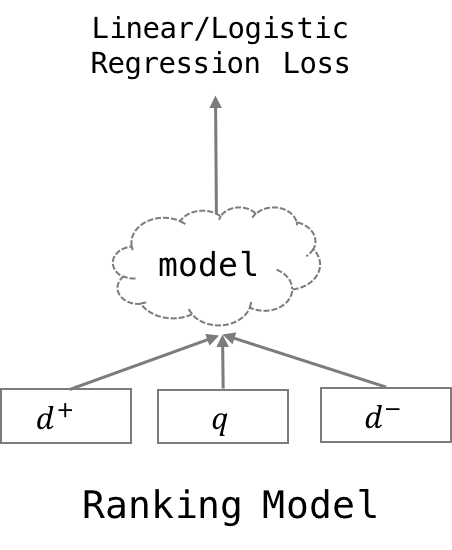
\includegraphics[height=2.7cm]{Images/O_n2_Models.png}
        \caption{\label{fig:o_n2_models}Quadratic time early combining model}
    \end{subfigure}%
\end{figure*}

